\documentclass{beamer}
\usepackage{beamerthemesplit}
\usepackage{wrapfig}
\usetheme{SPbGU}
\usepackage{pdfpages}
\usepackage{amsmath}
\usepackage{cmap} 
\usepackage[T2A]{fontenc} 
\usepackage[utf8]{inputenc}
\usepackage[english,russian]{babel}
\usepackage{indentfirst}
\usepackage{amsmath}
\usepackage{tikz}
\usepackage{multirow}
\usepackage[noend]{algpseudocode}
\usepackage{algorithm}
\usepackage{algorithmicx}
\usetikzlibrary{shapes,arrows}
\usepackage{fancyvrb}
\usepackage{epstopdf}
\newtheorem{rutheorem}{Свойство}
\newtheorem{ruproof}{Доказательство}
\newtheorem{rudefinition}{Определение}
\newtheorem{rulemma}{Лемма}
\beamertemplatenavigationsymbolsempty

\title[]{Синтаксический анализ регулярных множеств}
\institute[]{
Семинар научно-исследовательских лабораторий JetBrains }

\author[Екатерина Вербицкая]{Екатерина Вербицкая}

\date{21 ноября 2015г.}

\definecolor{orange}{RGB}{179,36,31}

\begin{document}
{

\begin{frame}
  \begin{center}
  {
\includegraphics[width=1cm]{SPbGU_Logo.png}}
  \end{center}
  \titlepage
\end{frame}
}

\begin{frame}[fragile]
  \transwipe[direction=90]
  \frametitle{Динамически формируемые выражения}
  \begin{itemize}
    \item \emph{Динамически формируемые выражения} генерируются из строковых литералов во время исполнения программы
    \begin{itemize}
      \item Также могут называться \emph{динамическим} или \emph{встроенным кодом}
    \end{itemize}
  \end{itemize}

  \begin{itemize}
    \item Программа, формирующая такие выражения --- \emph{генератор} или \emph{основная программа}
  \end{itemize}

  \begin{itemize}
    \item \emph{Точка интереса} --- строка основной программы, в которой осуществляется чтение значения формируемого выражения
  \end{itemize}

  \begin{itemize}
    \item \emph{Множество значений (динамического) выражения} --- множество всех выражений, 
которые могут породиться в процессе выполнения основной программы в данной точке интереса
  \end{itemize}

\end{frame}

\begin{frame}[fragile]
  \transwipe[direction=90]
  \frametitle{Динамически формируемые выражения: примеры}
  \begin{itemize}
    \item Встроенный SQL
      \begin{Verbatim}[commandchars=\\\{\}]
\textcolor{blue}{SqlCommand} myCommand = new \textcolor{blue}{SqlCommand}(
    \textcolor{orange}{"SELECT * FROM table WHERE Column = @Param2"},
    myConnection);
myCommand.Parameters.Add(myParam2);
      \end{Verbatim}

    \item Динамический SQL
      \begin{Verbatim}[commandchars=\\\{\}]
\textcolor{blue}{IF} @X = @Y
    \textcolor{blue}{SET} @TBL = \textcolor{orange}{' #table1 '}
\textcolor{blue}{ELSE}
    \textcolor{blue}{SET} @TBL = \textcolor{orange}{' table2 '}
\textcolor{blue}{SET} @S = \textcolor{orange}{'SELECT x FROM'} + @TBL + \textcolor{orange}{'WHERE ISNULL(n,0) > 1'}
EXECUTE (@S)
       \end{Verbatim}
    \end{itemize}
\end{frame}

\begin{frame}
  \transwipe[direction=90]
  \frametitle{Проблемы}  
  \begin{itemize}
    \item Встроенный код~--- код на некотором языке программирования, поэтому, как следствие, необходимы:
    \begin{itemize}
      \item Поддержка в IDE (подсветка кода, сообщение об ошибках, рефакторинги)
      \item Трансляция (миграция с устаревших технологий на новые платформы)
      \item Обнаружение уязвимостей
    \end{itemize}
  \end{itemize}
\end{frame}

\begin{frame}
  \transwipe[direction=90]
  \frametitle{Статический анализ встроенного кода}  
  \begin{itemize}
    \item Производится без выполнения основной программы
    \item Проверяет выполнение некоторых свойств для \emph{каждого} возможного выражения 
  \end{itemize}
  
  \begin{itemize}
    \item В общем случае задача статического анализа встроенных языков неразрешима 
    \item При \emph{регулярной аппроксимации} множества значений выражения некоторые задачи становятся разрешимыми
    \begin{itemize}
      \item \emph{Регулярная аппроксимация} --- аппроксимация (сверху) регулярным языком множества значений выражения 
    \end{itemize}
  \end{itemize}
\end{frame}

\begin{frame}
  \transwipe[direction=90]
  \frametitle{Существующие решения}
  \begin{itemize}
    \item PHP String Analyzer, Java String Analyzer, Alvor
    \begin{itemize}
      \item Статические анализаторы PHP, Java и SQL, встроенных в Java 
    \end{itemize}

    \item Kyung-Goo Doh et al.
    \begin{itemize}
      \item Проверяет синтаксическую корректность встроенного кода
    \end{itemize}

    \item PHPStorm
    \begin{itemize}
      \item IDE для PHP с поддержкой HTML, CSS, JavaScript
    \end{itemize}

    \item IntelliLang
    \begin{itemize}
      \item PHPStorm и IDEA plugin, поддержка многих языков
    \end{itemize} 

    \item STRANGER
    \begin{itemize}
      \item Обнаружение уязвимости в коде на PHP
    \end{itemize}
  \end{itemize}
  
  \begin{itemize}
    \item Недостатки
    \begin{itemize}
      \item Ограниченная функциональность
      \item Сложно расширить новой функциональностью или поддержать новые языки
      \item Не создают структурного представления динамического кода
    \end{itemize}
  \end{itemize}
\end{frame}


\begin{frame}
  \transwipe[direction=90]
  \frametitle{Статический анализ встроенных языков: схема}
  \begin{itemize}
    \item Определение точек интереса
    \item Построение аппроксимации
    \item Лексический анализ
    \item \textbf{Синтаксический анализ}
    \begin{itemize}
      \item Относительно эталонной грамматики
    \end{itemize}
    \item Семантический анализ
  \end{itemize}
\end{frame}



\begin{frame}[fragile]
\transwipe[direction=90]
\frametitle{Статический анализ встроенных языков: схема}

\begin{tabular}{p{5.0cm} p{8cm}}
Код: выделена точка интереса
&
\begin{minipage}[t]{5cm}

\begin{Verbatim}[commandchars=\\\{\}]
\textcolor{blue}{string} res = \textcolor{orange}{""};
\textcolor{blue}{for}(i = 0; i < l; i++)
    res = \textcolor{orange}{"()"} + res;
\fbox{\textcolor{blue}{use}(res);}

\end{Verbatim}
\end{minipage}

\\ 
Порождаемые значения
&
\begin{minipage}[t]{2.5cm}
\begin{Verbatim}[commandchars=\\\{\}]
\{\textcolor{orange}{""}, \textcolor{orange}{"()"},  \textcolor{orange}{"()()"}, ..., \textcolor{orange}{"()"}^l\}
\end{Verbatim}
\end{minipage}

\\
Регулярная аппроксимация
&
\begin{minipage}[t]{4cm}
  \begin{Verbatim}[commandchars=\\\{\}]
(\textcolor{orange}{"()"})*
  \end{Verbatim} 
\end{minipage}

\\
Аппроксимация
&
\begin{minipage}[t]{3cm}
\raisebox{-\height}{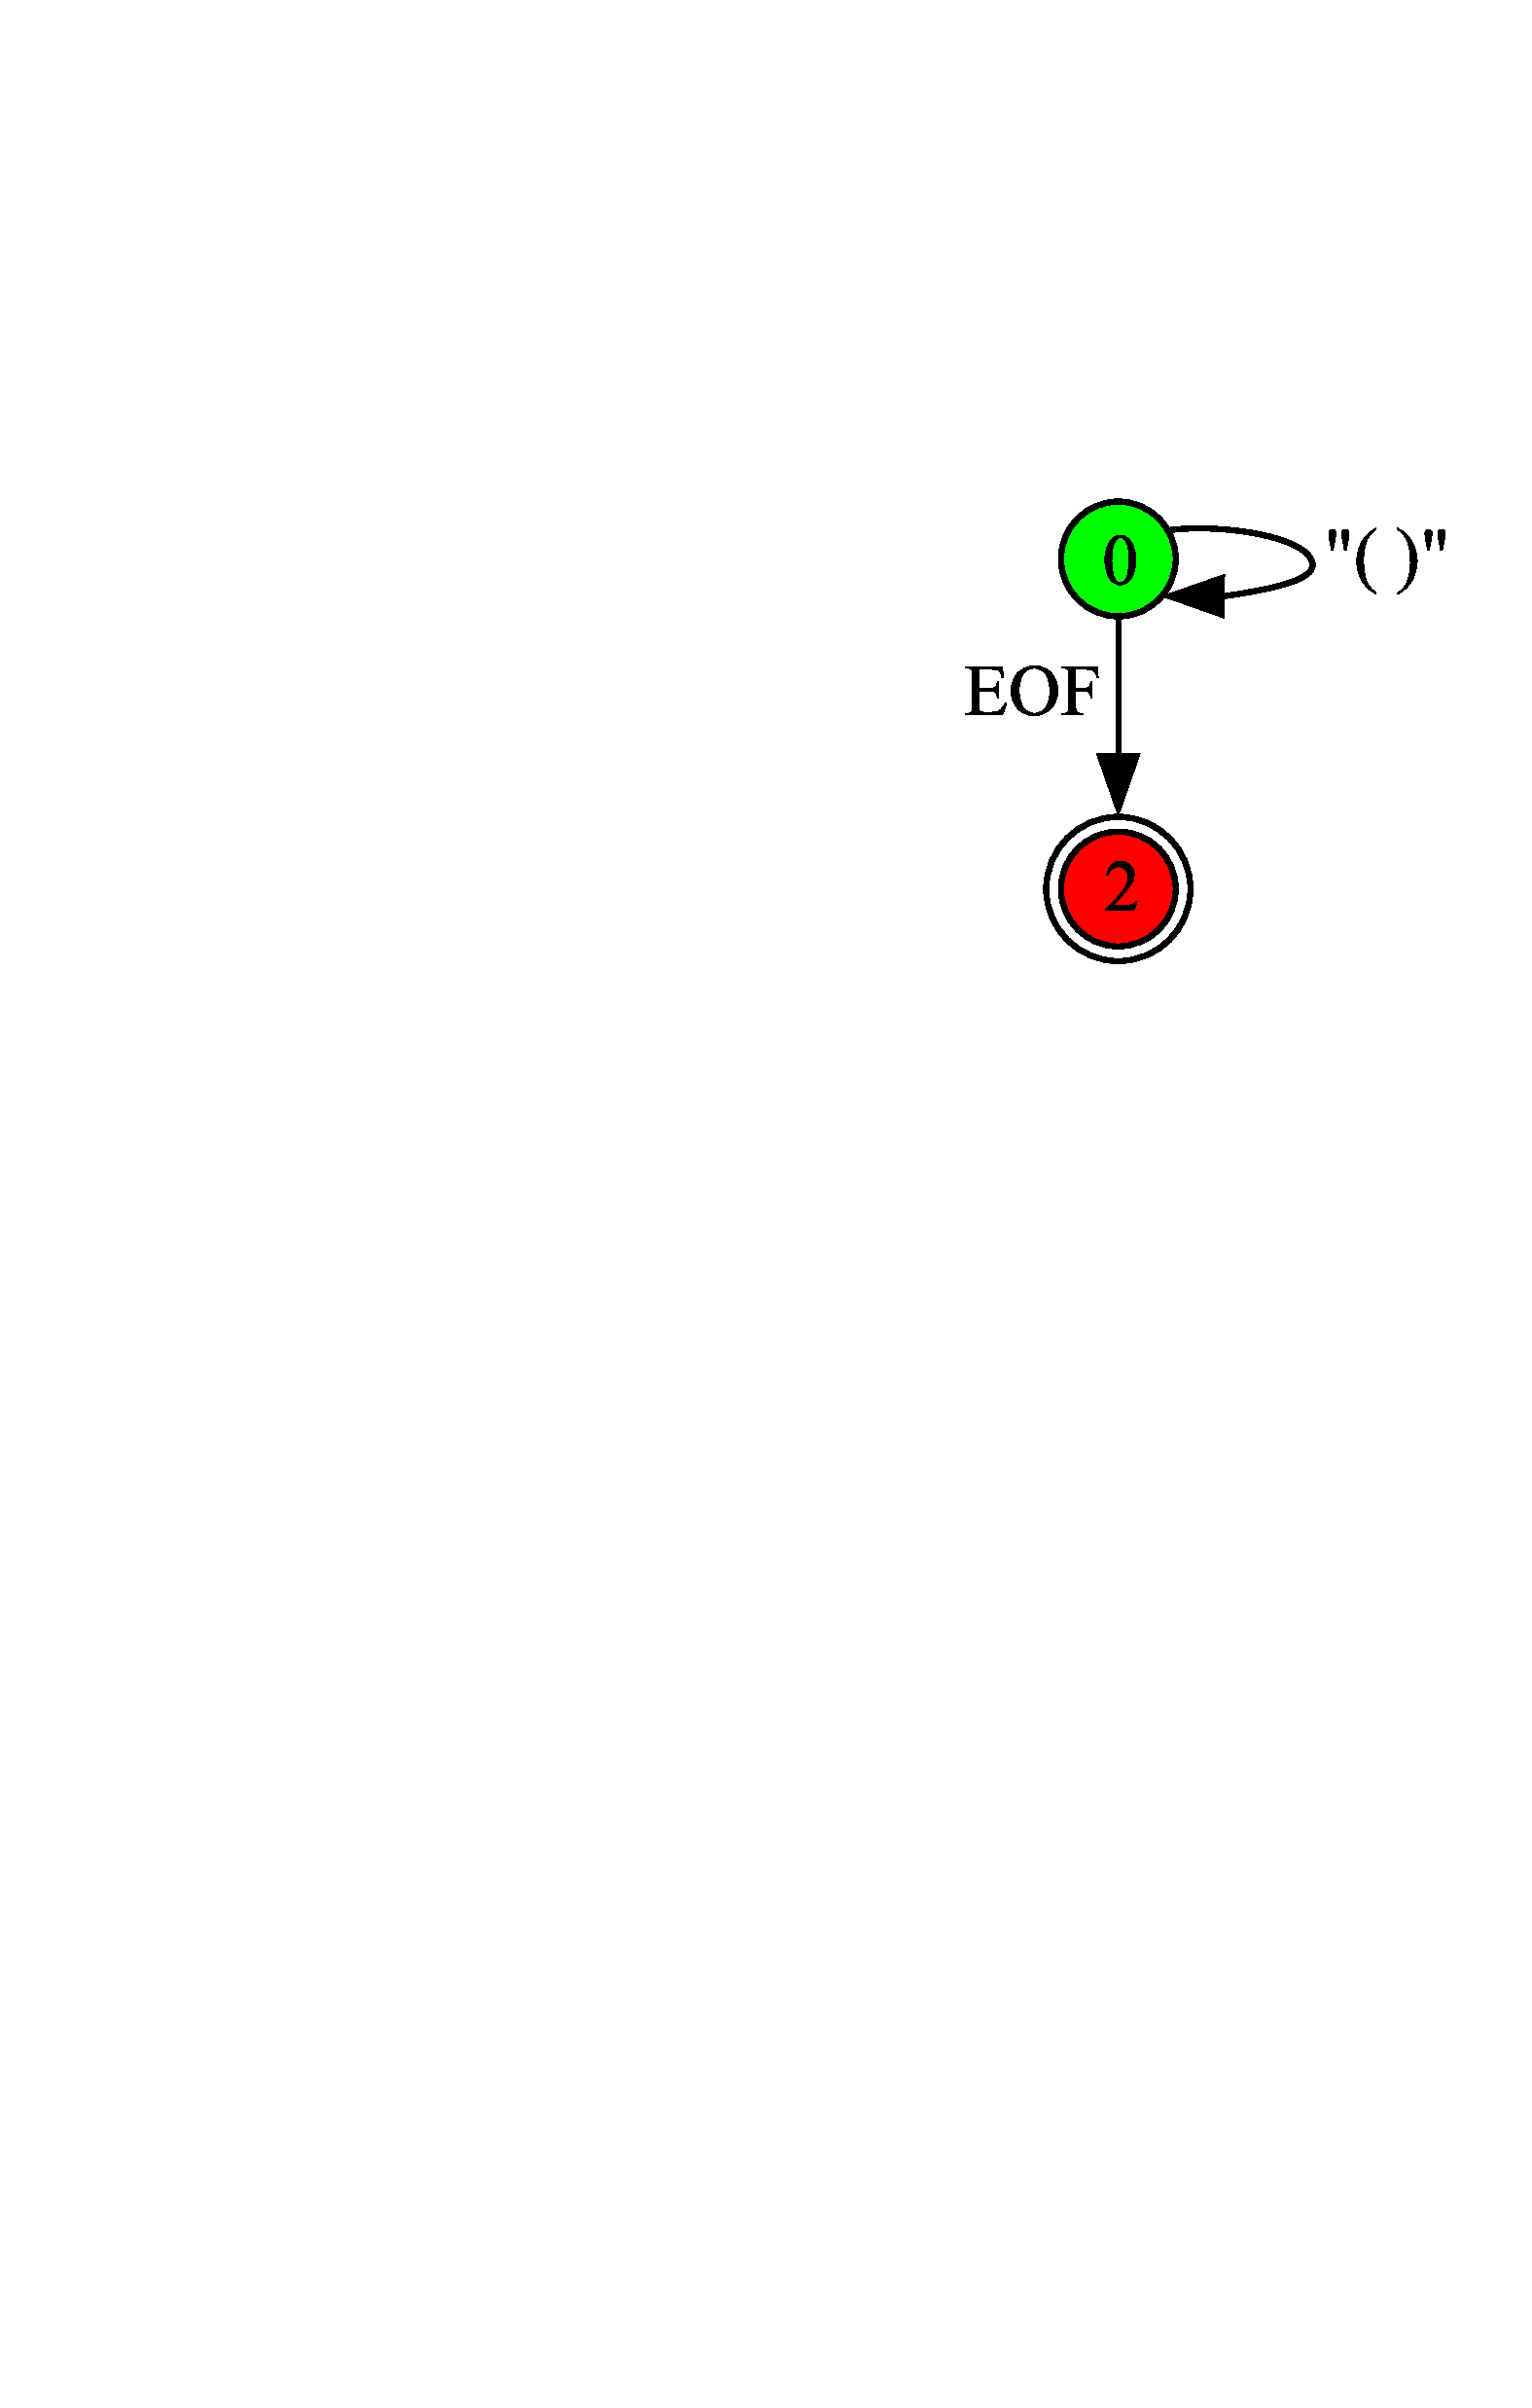
\includegraphics[width=2cm]{pictures/lex1}}
\end{minipage}


\end{tabular}


\end{frame}


\begin{frame}[fragile]
\transwipe[direction=90]
\frametitle{Статический анализ встроенных языков: схема}

\begin{tabular}{p{4.5cm} p{8cm}}
\begin{minipage}[t]{4cm}
Аппроксимация\\
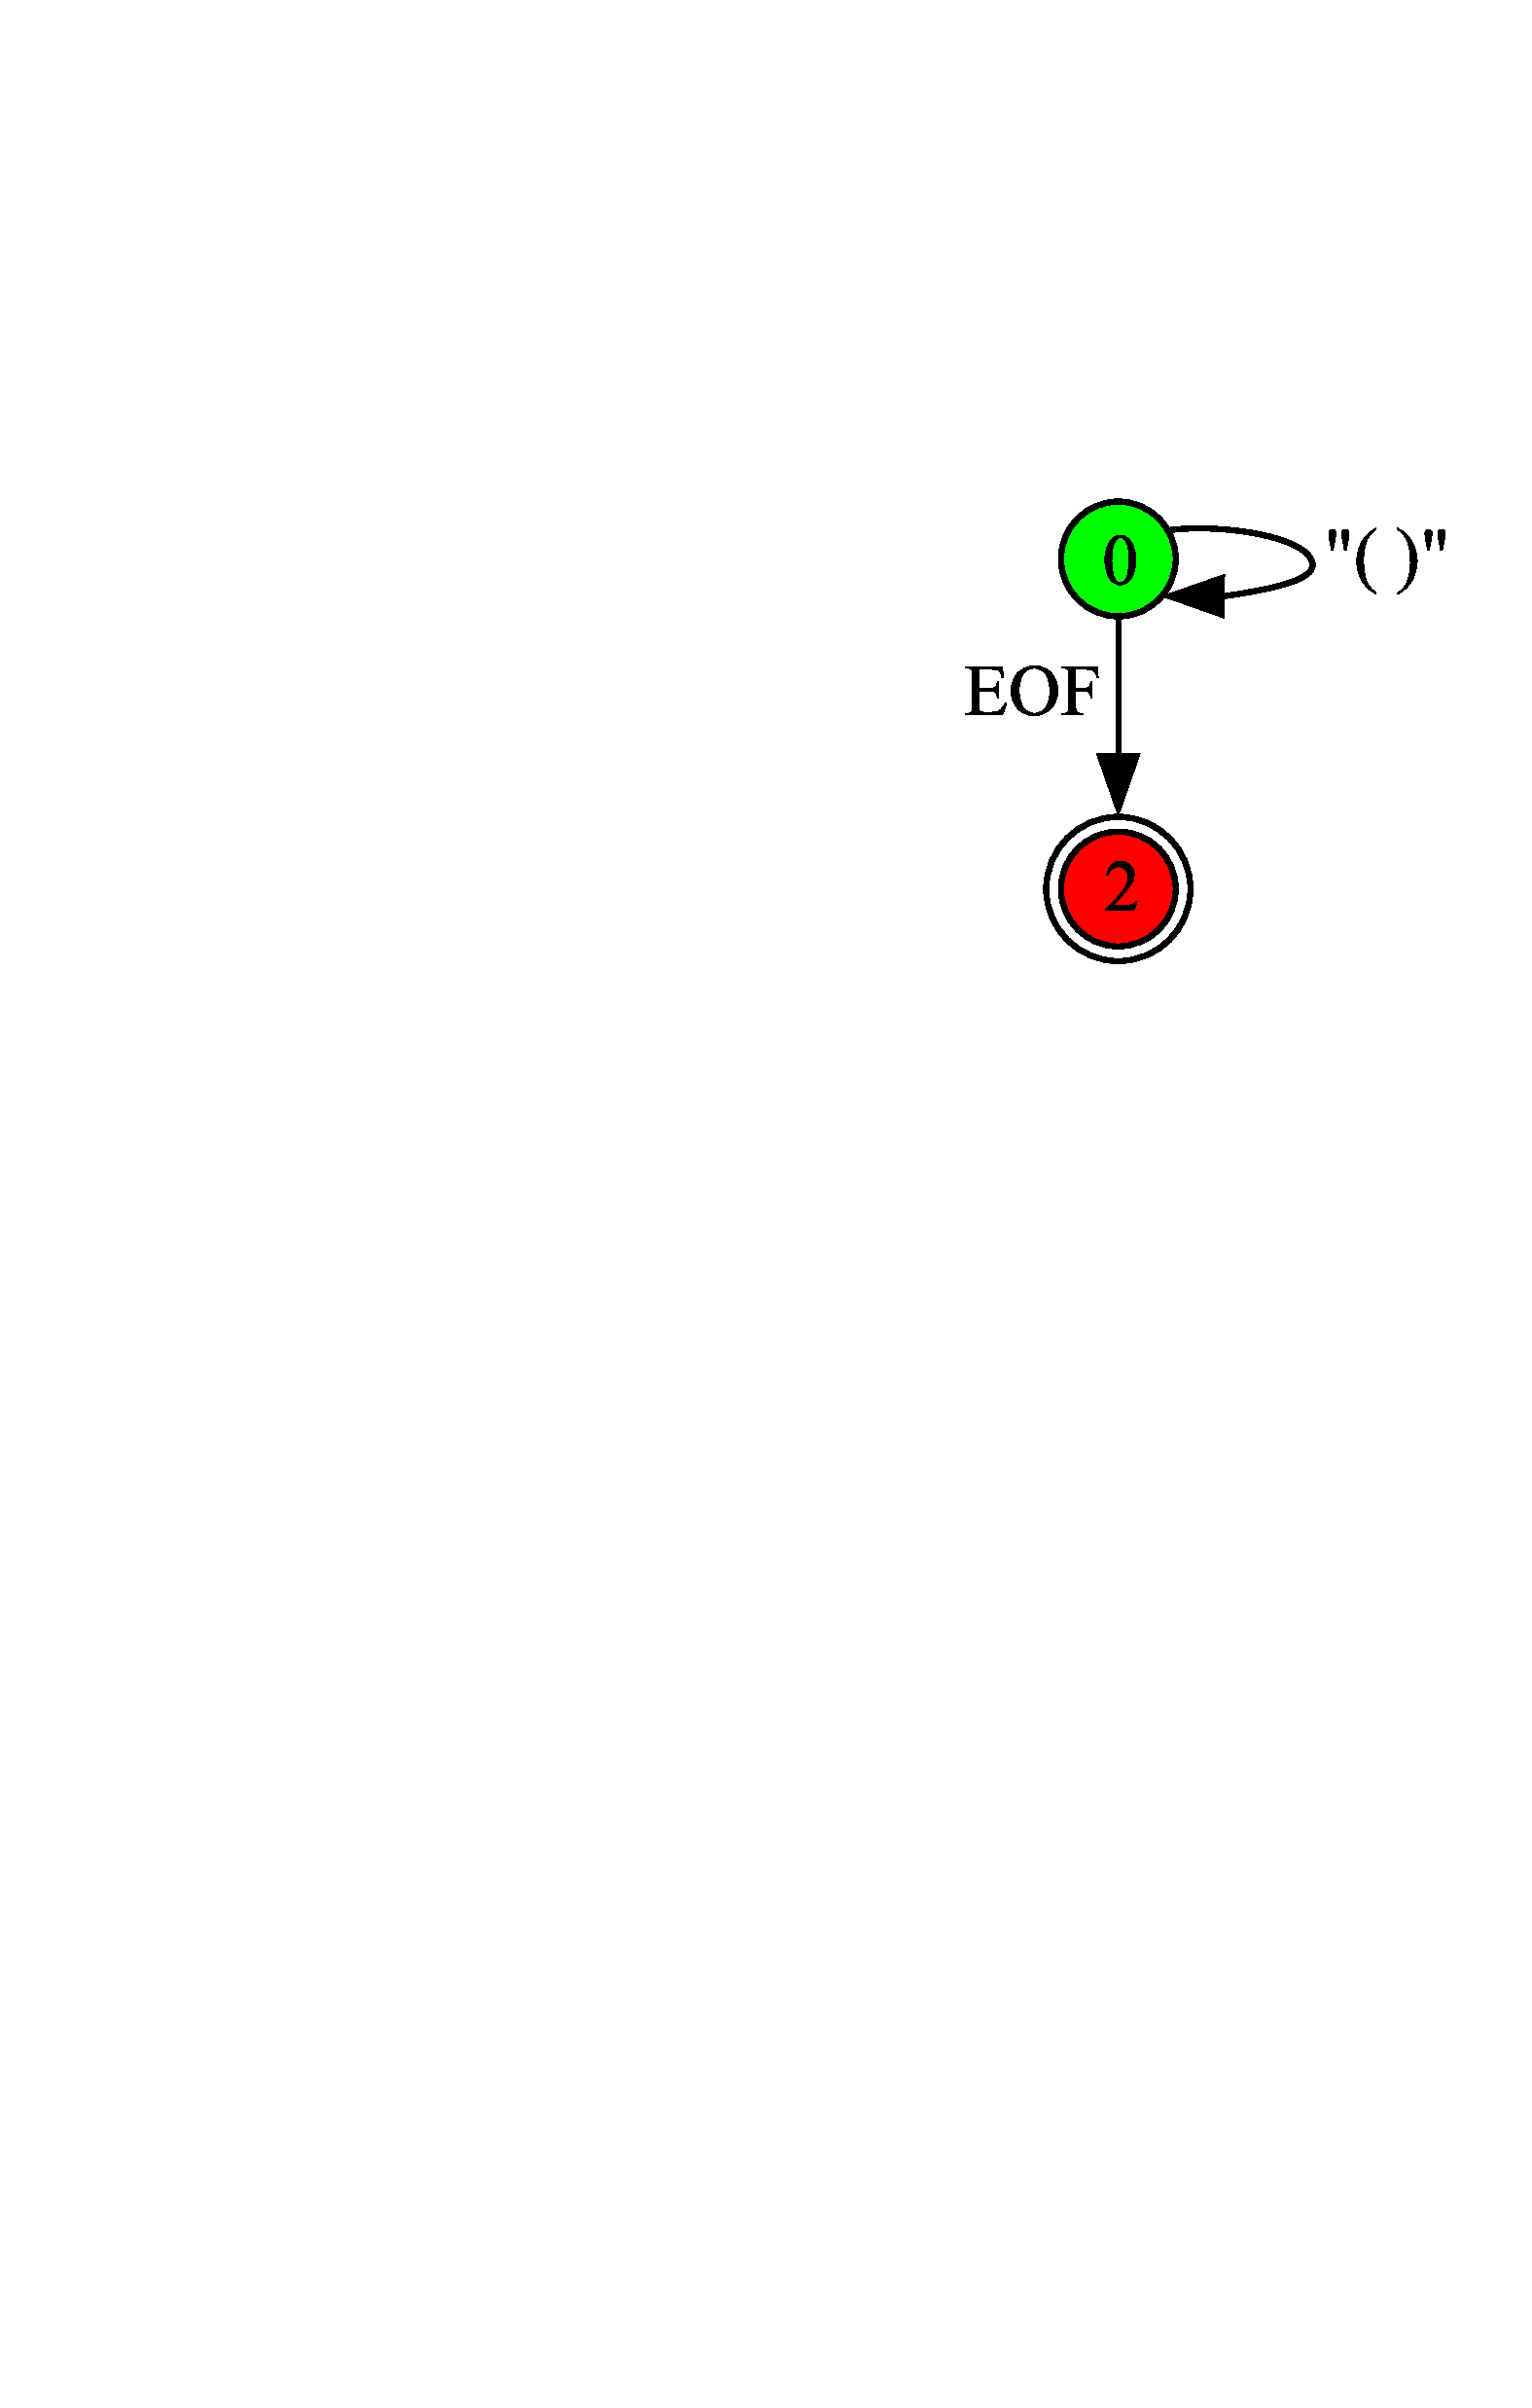
\includegraphics[width=2cm]{pictures/lex1}

После лексического анализа\\
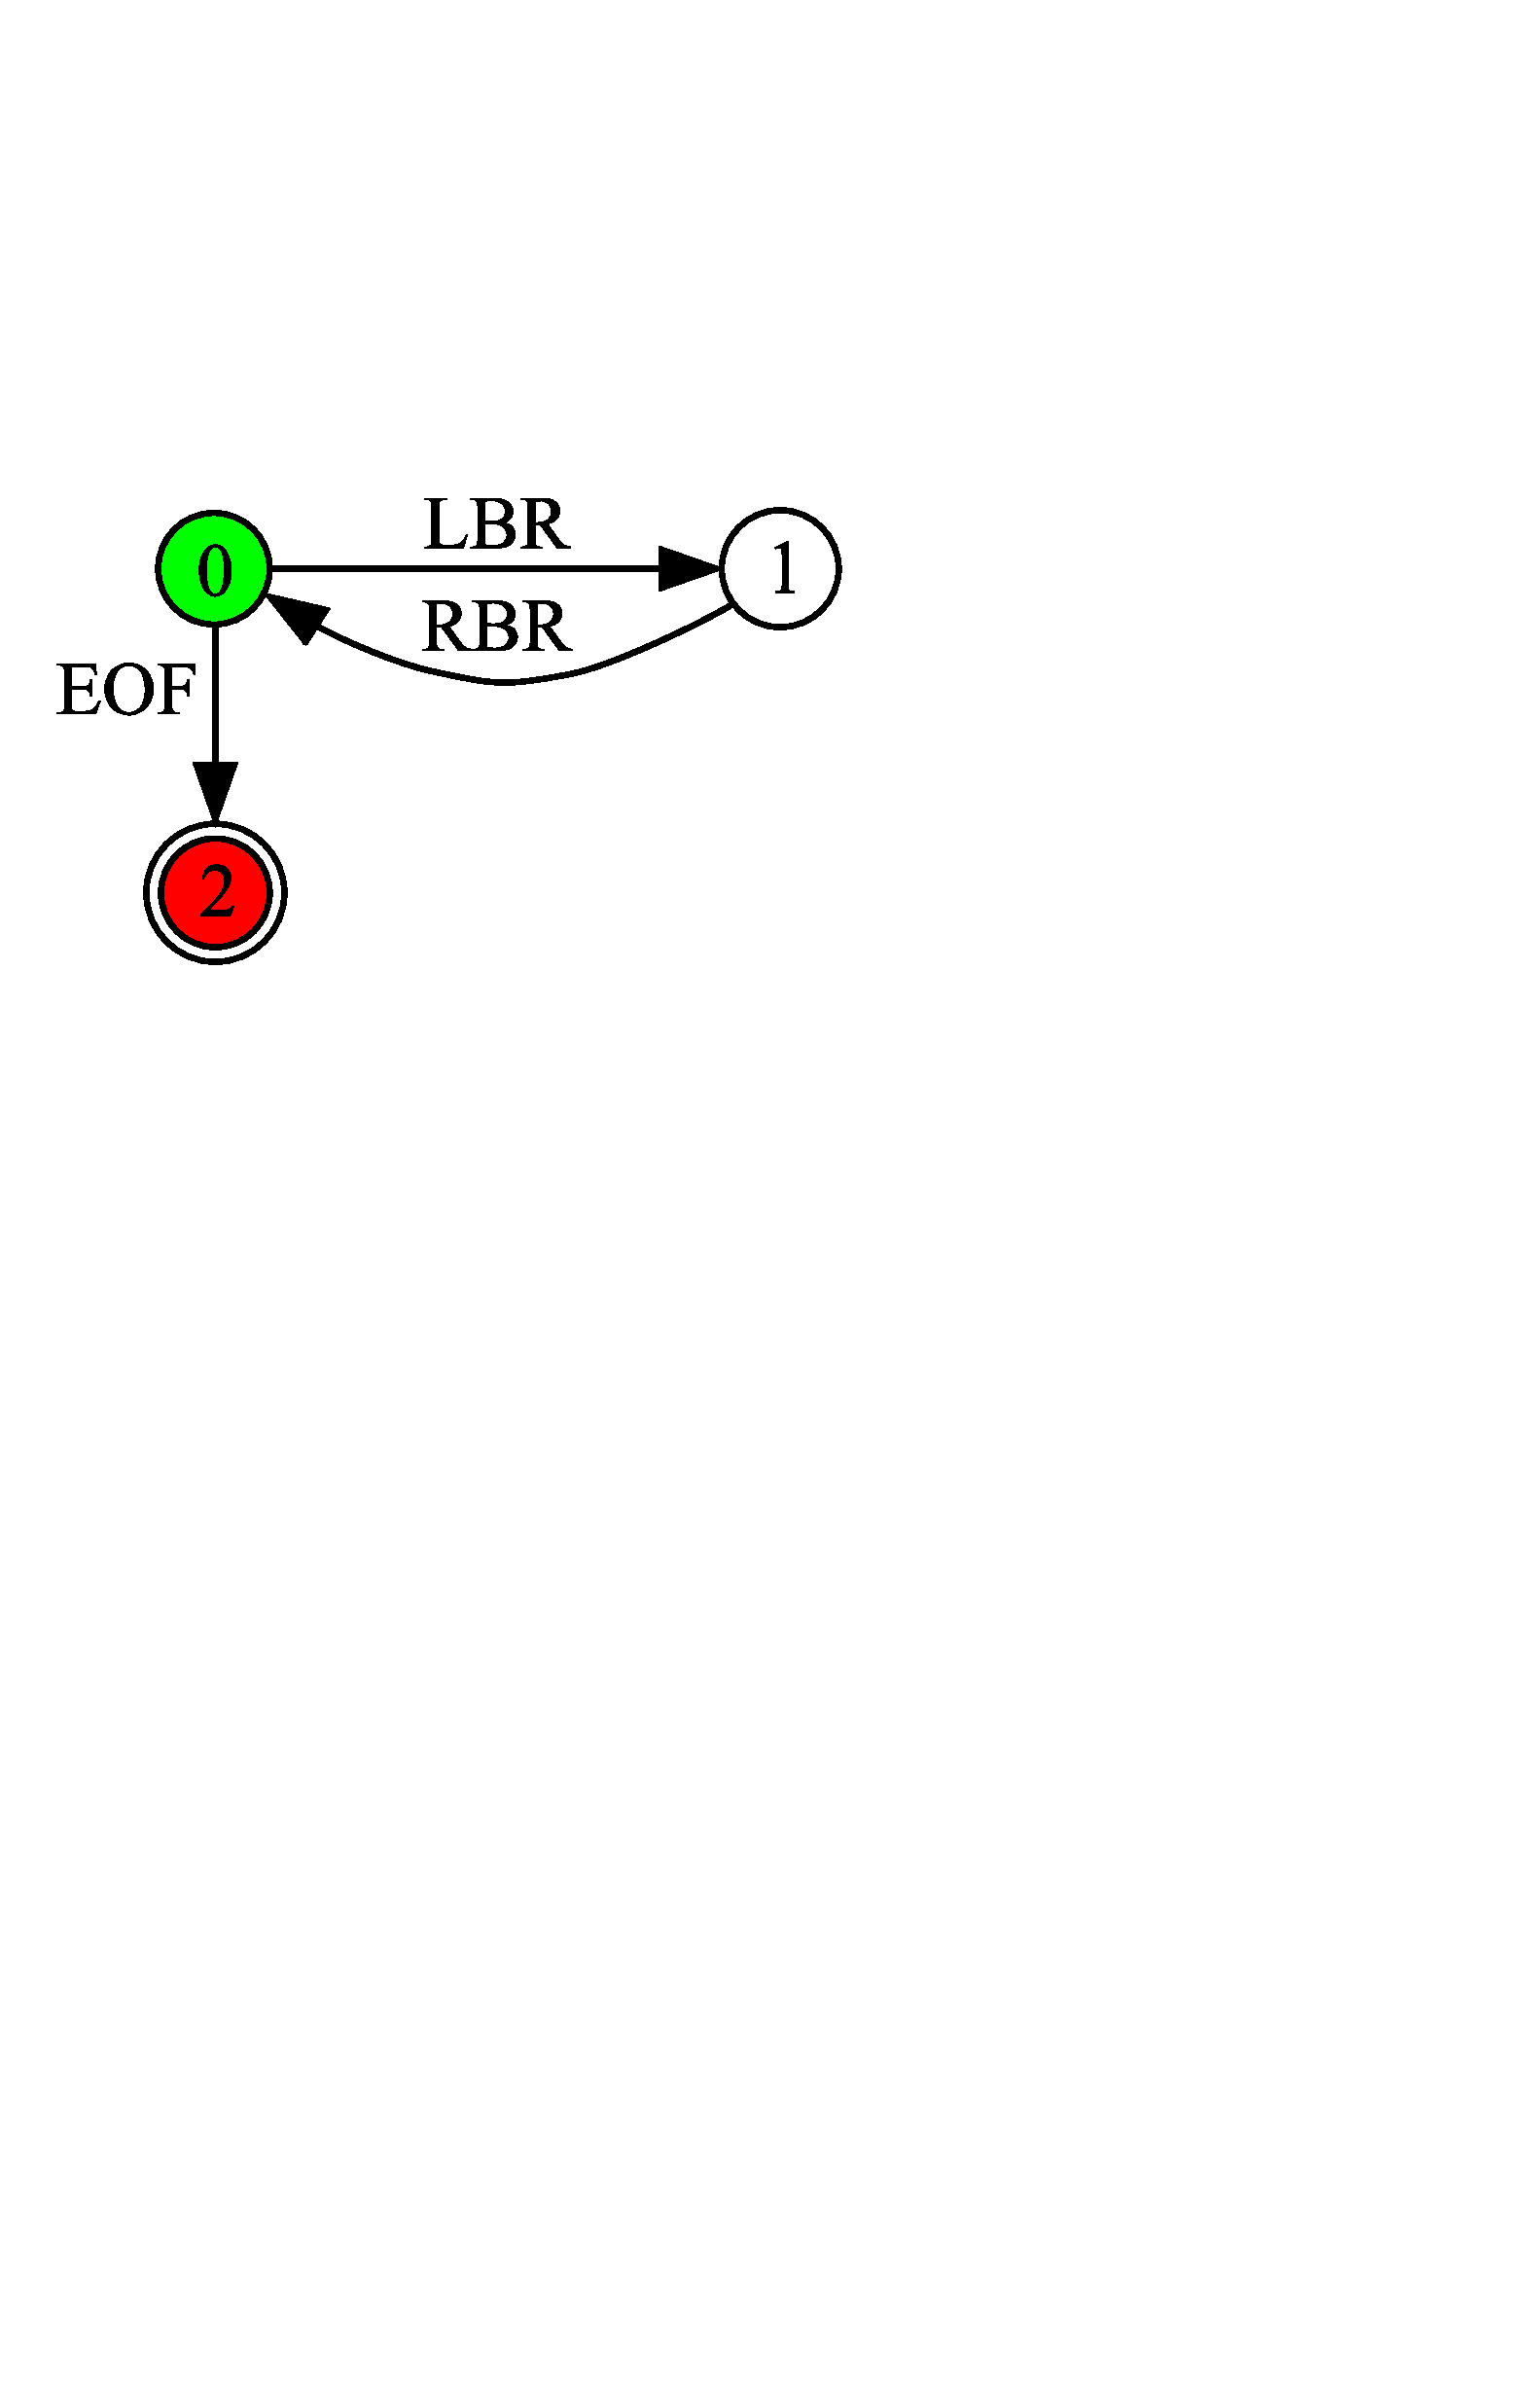
\includegraphics[width=3cm]{pictures/in31}

Грамматика\\
\vspace{-5pt}
$$
\begin{array}{crcl}
&start &::=& s \\
&s & ::= & \mbox{\texttt{LBR }} s \mbox{\texttt{ RBR }} s\\
&s & ::= &\epsilon
\end{array}
$$
\end{minipage}
&

\begin{minipage}[t]{8cm}
Лес разбора\\
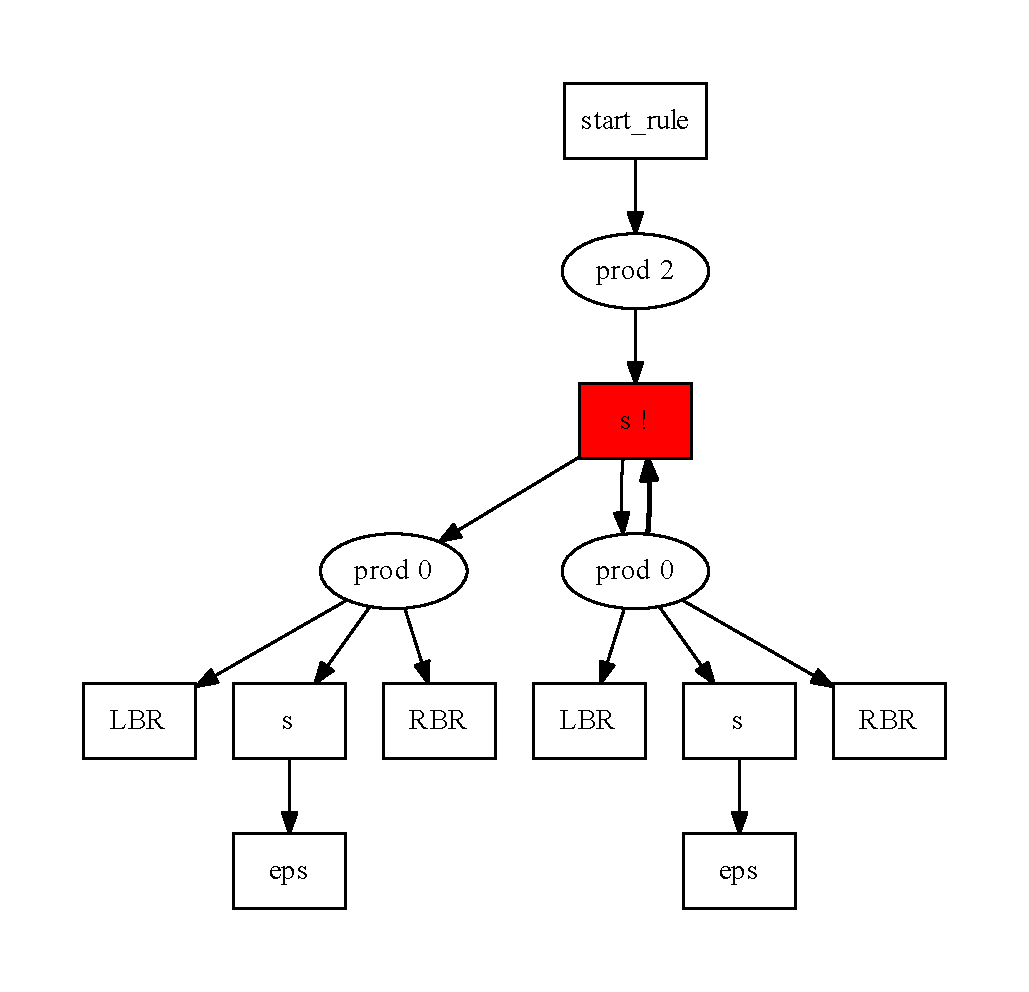
\includegraphics[width=7cm]{pictures/out3}
\end{minipage}

\end{tabular}

\end{frame}

\begin{frame}
  \transwipe[direction=90]
  \frametitle{Постановка задачи}
  \textbf{Цель:} разработать алгоритм, подходящий для синтаксического анализа 
встроенного кода

  \begin{itemize}
    \item \emph{Синтаксический анализ} --- сопоставление каждого выражения из 
апроксимирующего языка с некоторой эталонной грамматикой и построение деревьев разбора
  \end{itemize}
\end{frame}  

\begin{frame}
  \transwipe[direction=90]
  \frametitle{Постановка задачи}
  \textbf{Задачи}:
  \begin{itemize}
    \item Разработать алгоритм для синтаксического анализа регулярного языка, который строит конечный лес разбора
    \item Лес разбора должен содержать дерево разбора для каждой корректной строки из регулярного языка
    \item Диагностики ошибок не предусматривается: некорректные выражения игнорируются
    \item Алгоритм не должен зависеть от языков основной программы и встроенного кода
  \end{itemize}
\end{frame}
            
\begin{frame}
  \transwipe[direction=90]
  \frametitle{Алгоритм}
  \begin{itemize}
    \item \textbf{Входные данные} 
      \begin{itemize} 
        \item Эталонная КС грамматика $G$
        \item Регулярный язык в виде графа ДКА без $\epsilon$-переходов над алфавитом терминалов грамматики $G$
      \end{itemize}
    \item \textbf{Результат}
      \begin{itemize} 
        \item Лес разбора всех корректных выражений, принимаемых входным автоматом
    \end{itemize}
  \end{itemize}
\end{frame}

\begin{frame}
  \transwipe[direction=90]
  \frametitle{Right-Nulled Generalized LR алгоритм}
  \begin{itemize}
    \item RNGLR обрабатывает произвольные КС грамматики
    \item Табличный синтаксический анализ 
    \item В случае LR-конфликтов, продолжает обработку всех возможных вариантов
    \begin{itemize}
      \item Shift/Reduce конфликт
      \item Reduce/Reduce конфликт
    \end{itemize}
    \item Использует специальные структуры данных, ограничивающие потребление 
памяти и гарантирующие полиномиальное время работы
  \end{itemize}
\end{frame}

\begin{frame}
  \transwipe[direction=90]
  \frametitle{Структуры данных: Graph-Structured Stack}
  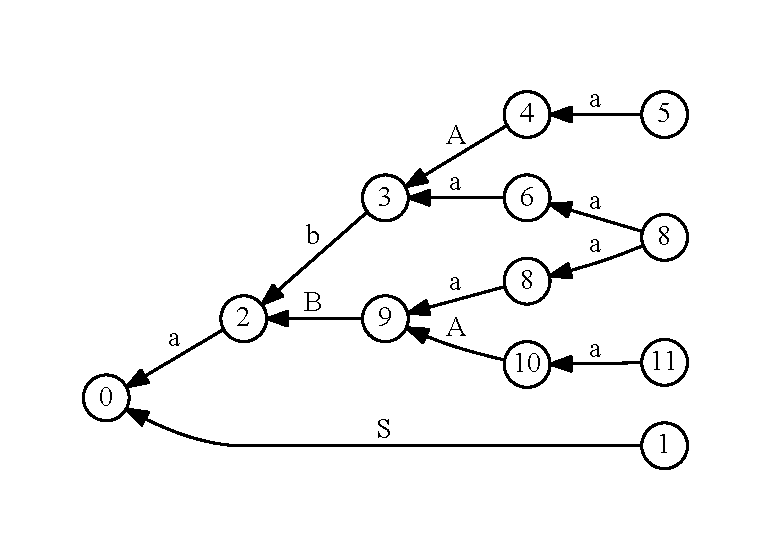
\includegraphics[width=12cm]{pictures/gss_rnglr}
\end{frame}

\begin{frame}
  \transwipe[direction=90]
  \frametitle{Операции в RNGLR-алгоритме: shift (сдвиг)}
  \begin{center}
  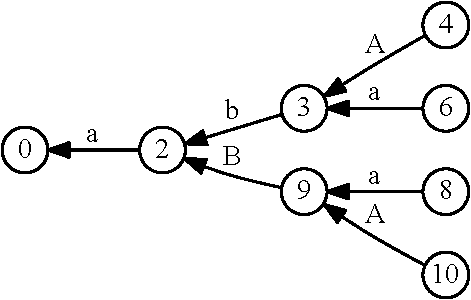
\includegraphics[width=6cm]{pictures/gss_rnglr_shift_1} \\ \vspace{10pt} 
  \pause
  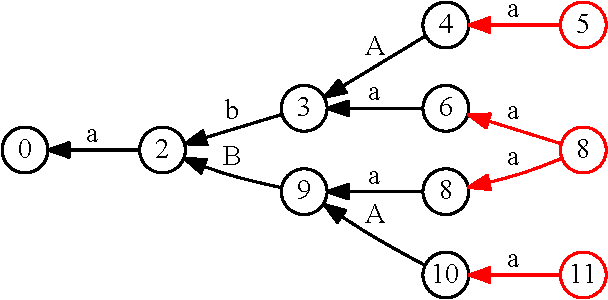
\includegraphics[width=6cm]{pictures/gss_rnglr_shift_2}
  \end{center}
\end{frame}

\begin{frame}
  \transwipe[direction=90]
  \frametitle{Операции в RNGLR-алгоритме: reduce (редукция или свертка)}
  \begin{center}
  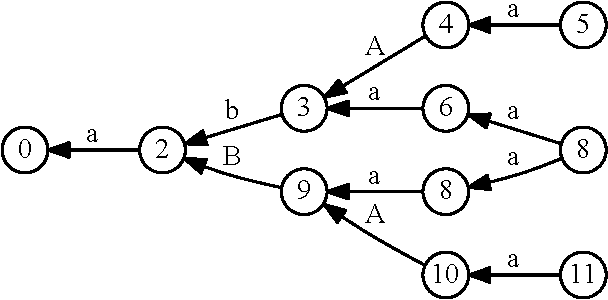
\includegraphics[width=6cm]{pictures/gss_rnglr_reduce_1} \\  \vspace{10pt}
  \pause
  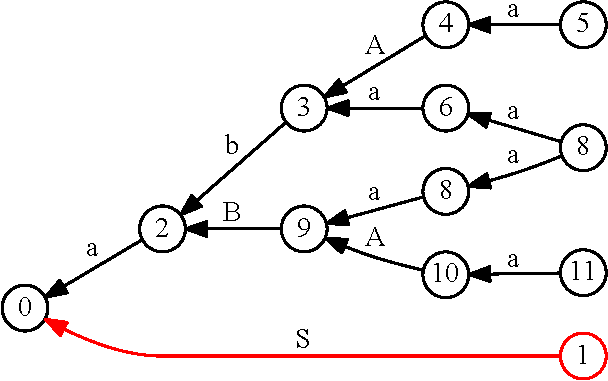
\includegraphics[width=6cm]{pictures/gss_rnglr_reduce_2}
  \end{center}
\end{frame}

\begin{frame}
  \transwipe[direction=90]
  \frametitle{RNGLR}
  \begin{itemize}
    \item Входной поток читается последовательно
    \begin{itemize}
      \item Обработать все редукции
      \item Сдвинуть следующий символ со входа
    \end{itemize}
  \end{itemize}
  \begin{itemize}
    \item При добавлении новой вершины в GSS вычисляется сдвиг
    \item При добавлении нового ребра --- редукции
  \end{itemize}
\end{frame}



\begin{frame}
  \transwipe[direction=90]
  \frametitle{Алгоритм}
  \begin{itemize}
    \item GSS строится последовательно во время обхода графа входного автомата, 
похожим образом, что в RNGLR
    \item Новый тип ``конфликта'': Shift/Shift
  \end{itemize}
  \begin{itemize}
    \item Множество LR-состояний ассоциируется с каждой вершиной входного графа
    \item Порядок, в котором обходятся вершины входного графа, определяется 
очередью. Каждый раз, когда ребро добавляется в GSS, его начальная вершина 
добавляется в очередь
  \end{itemize}
  \begin{itemize}
    \item Обнаружения ошибок не производится, некорректные строки игнорируются
  \end{itemize}
\end{frame}

\begin{frame}
  \transwipe[direction=90]
  \frametitle{Обработка циклов: начальный стек}
  \begin{center}                                
  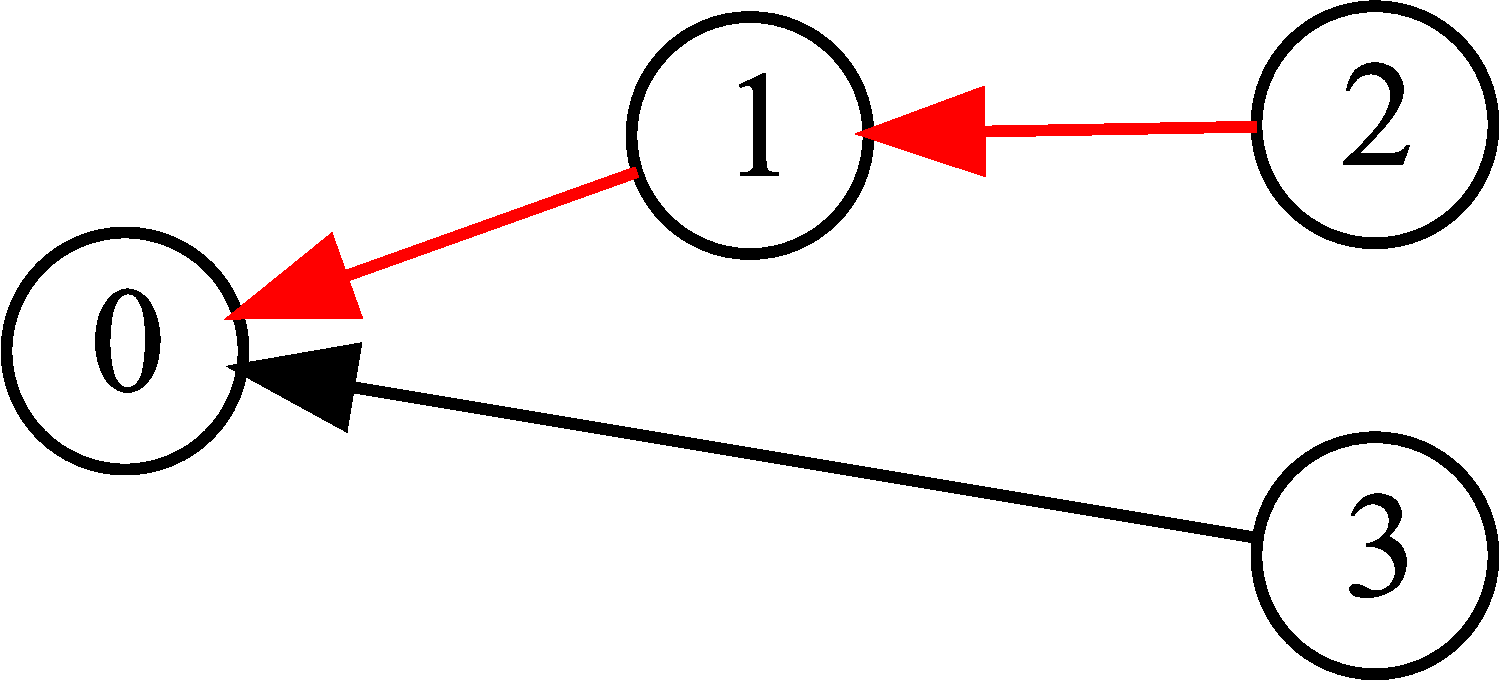
\includegraphics[width=6cm]{pictures/gss_cycle/gss_cycle_init_highlight}
  \end{center}
\end{frame}

\begin{frame}
  \transwipe[direction=90]
  \frametitle{Обработка циклов: добавили несколько ребер}
  \begin{center}                                
  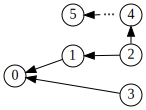
\includegraphics[width=6cm]{pictures/gss_cycle/gss_cycle_no_square}
  \end{center}
\end{frame}

\begin{frame}
  \transwipe[direction=90]
  \frametitle{Обработка циклов: образовался цикл}
  \begin{center}                                
  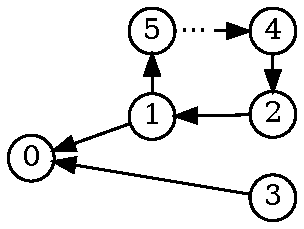
\includegraphics[width=6cm]{pictures/gss_cycle/gss_cycle_no_red_no_highlight}
  \end{center}
\end{frame}

\begin{frame}
  \transwipe[direction=90]
  \frametitle{Обработка циклов: новая редукция}
  \begin{center}                                
  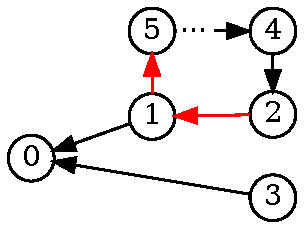
\includegraphics[width=6cm]{pictures/gss_cycle/gss_cycle_no_red}
  \end{center}
\end{frame}

\begin{frame}
  \transwipe[direction=90]
  \frametitle{Обработка циклов: добавили новую редукцию}
  \begin{center}                                
  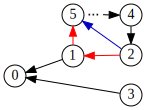
\includegraphics[width=6cm]{pictures/gss_cycle/gss_cycle}
  \end{center}
\end{frame}

\begin{frame}
  \transwipe[direction=90]
  \frametitle{Построение леса разбора}
  \begin{itemize}
    \item Shared Packed Parse Forest~--- граф, в котором объединено множество 
деревьев вывода
    \item Строится так же, как в RNGLR-алгоритме
    \end{itemize}
    \begin{itemize}
      \item С каждым ребром GSS ассоциируется фрагмент дерева вывода
      \item При обработке shift, создается дерево из одной вершины, 
соответствующей терминалу
      \item При обработке reduce, создается дерево, детьми корня которого 
становятся деревья, ассоциированные с ребрами путей
      \begin{itemize}
        \item Фрагменты деревьев переиспользуются, не копируясь
      \end{itemize}
      \item Корень результирующего леса разбора ассоциирован с ребром GSS, 
соответствующим свертке к стартовому нетерминалу
      \begin{itemize}
        \item Все недостижимые вершины удаляются из графа-леса
      \end{itemize}
    \end{itemize}

\end{frame}

\begin{frame}
\transwipe[direction=90]
\frametitle{Корректность алгоритма}
\begin{tabular}{p{5.3cm} p{6.7cm}}
\emph{Корректное дерево}~--- дерево вывода строки, накопленной вдоль 
некоторого пути во входном графе
&
\\
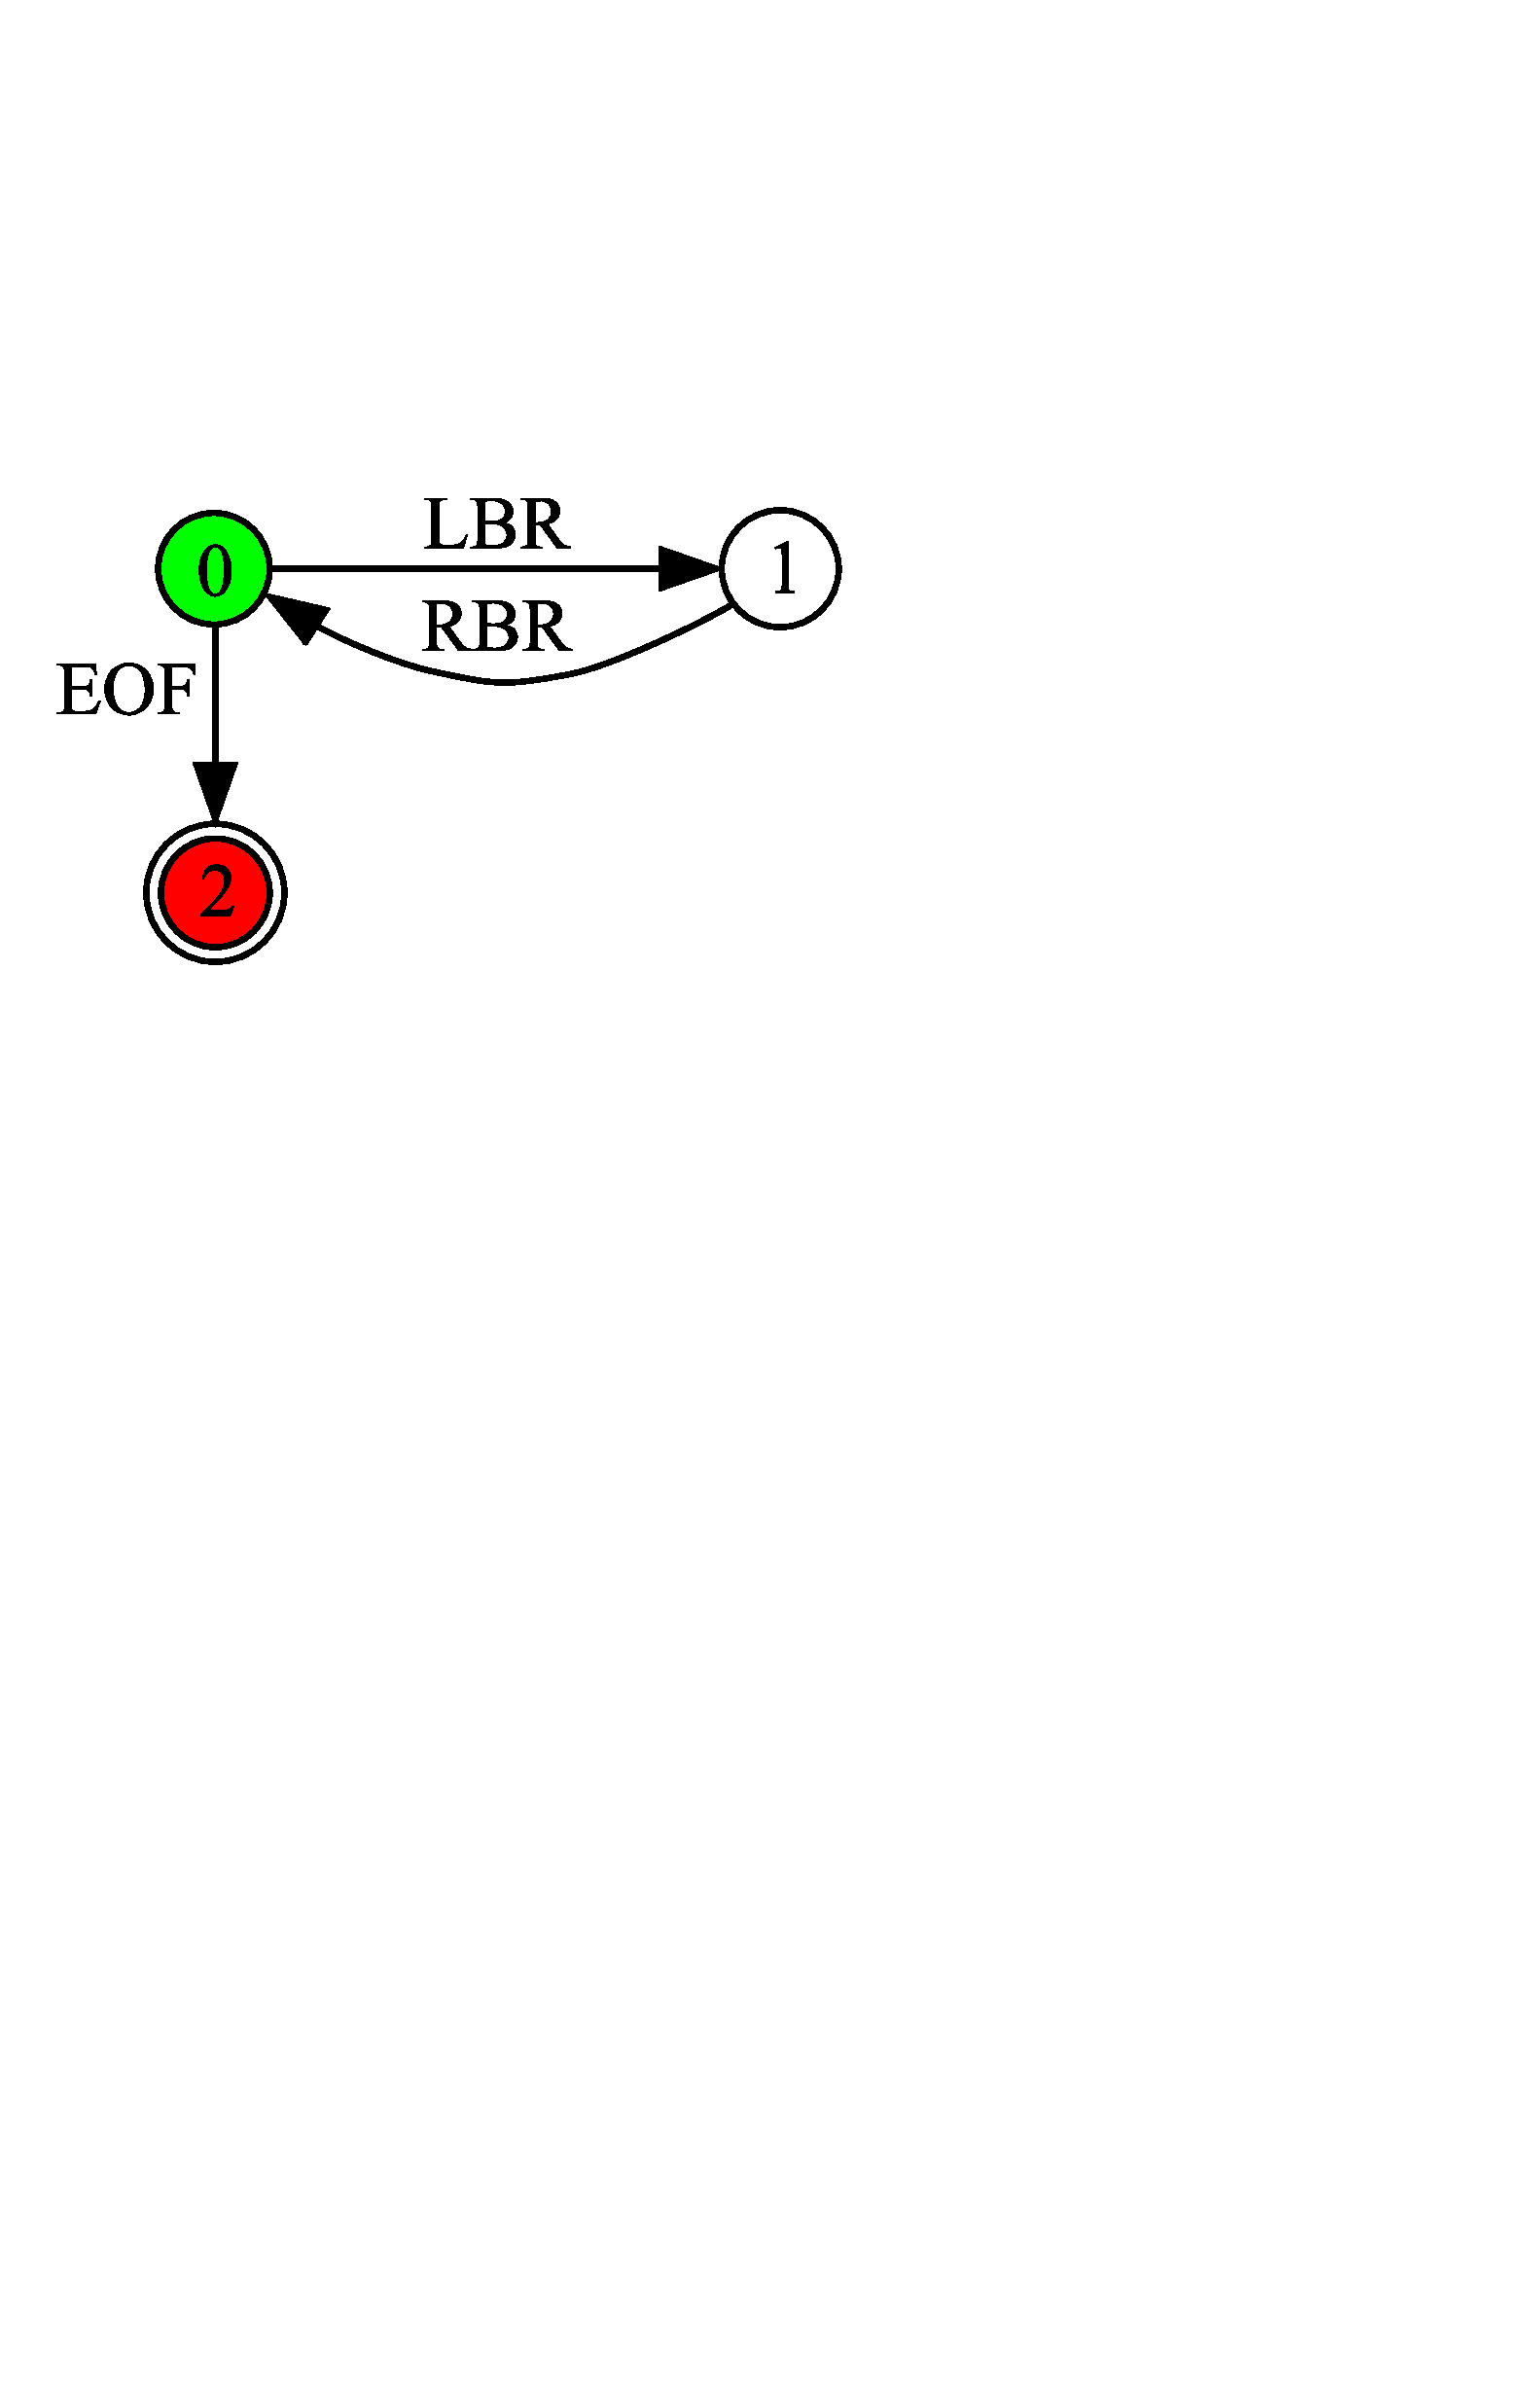
\includegraphics[width=5cm]{pictures/in31.pdf}
&
\includegraphics[width=6cm]{pictures/sppf2.eps}
\end{tabular}
\end{frame}


\begin{frame}
  \transwipe[direction=90]
  \frametitle{Алгоритм: корректность}
  \begin{rutheorem}[Завершаемость]
  \normalfont	
    Алгоритм завершается при любом входе
  \end{rutheorem}
  
  \begin{rutheorem}[Корректность]
  \normalfont  
    Каждое дерево, генерируемое из SPPF, корректно
  \end{rutheorem}

  \begin{rutheorem}[Корректность]
  \normalfont
    Для каждой строки из входного регулярного множества, корректной 
относительно эталонной грамматики, из SPPF можно извлечь корректное дерево 
  \end{rutheorem}
\end{frame}

\begin{frame}
  \transwipe[direction=90]
  \frametitle{Реализация}
  \begin{itemize}
    \item Алгоритм реализован как часть проекта YaccConstructor на языке 
программирования F\#
    \item Генератор таблиц RNGLR и описание структур данных GSS и SPPF 
переиспользованы
 \end{itemize}
\end{frame}

\begin{frame}[t]
  \transwipe[direction=90]
  \frametitle{Тестирование}
  \begin{itemize}
    \item Данные взяли из промышленного проекта по миграции с MS-SQL на Oracle Server 
    \item Всего 2,7 млн. строк кода, 2430 запросов, 2188 успешно обработаны
    \item С 45 до 1 сократилось количество необработанных запросов
  \end{itemize}
  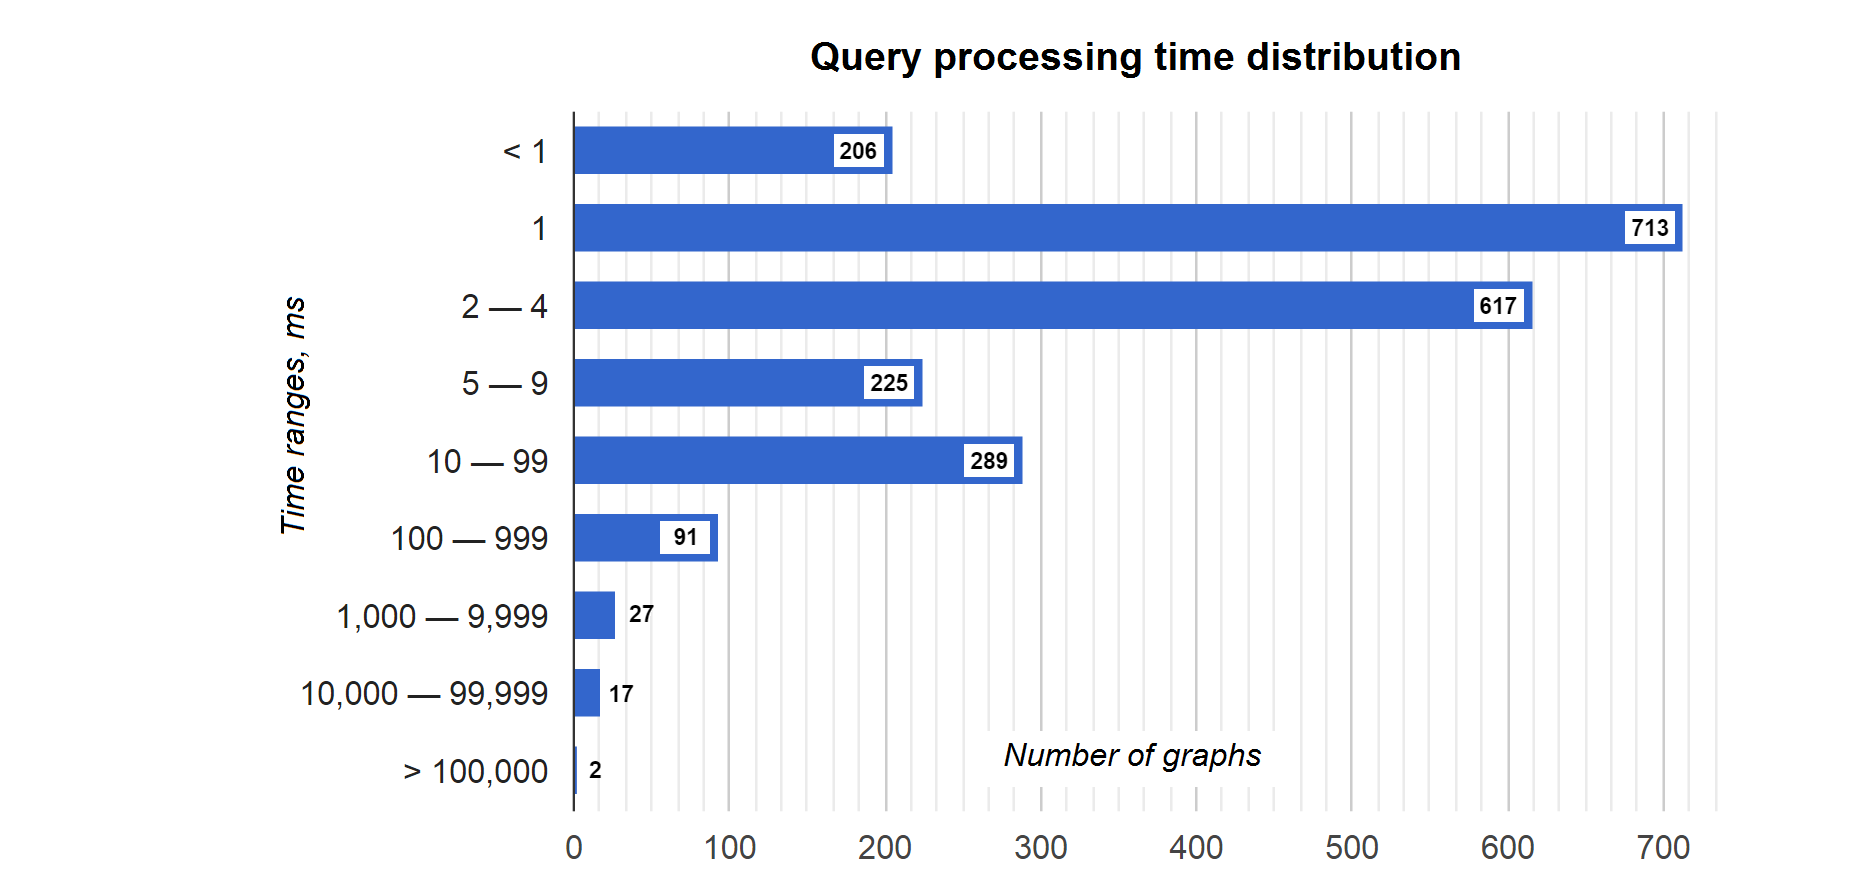
\includegraphics[width=10cm]{pictures/dist.png}
\end{frame}


\begin{frame}
  \transwipe[direction=90]
  \frametitle{Заключение}
  \begin{itemize}
    \item Разработан алгоритм синтаксического анализа регулярной аппроксимации 
динамически формируемых выражений, который строит конечное представление леса 
разбора 
    \item Доказаны завершаемость и корректность алгоритма
    \item Алгоритм реализован как часть проекта YaccConstructor
    \begin{itemize}
      \item \url{https://github.com/YaccConstructor/YaccConstructor}
    \end{itemize}
    \item Продемонстрирована применимость алгоритма для решения 
сложных задач
  \end{itemize}
\end{frame}

\begin{frame}
  \transwipe[direction=90]
  \frametitle{Настоящее и будущее}
  \begin{itemize}
    \item Обнаружение ошибок и сообщение о них
    \item Теоретическая оценка сложности
    \item Вычисление семантики над полученным лесом разбора
    \item Интеграция в плагин к ReSharper
  \end{itemize}
\end{frame}


\end{document}